\newcommand{\NWtarget}[2]{\hypertarget{#1}{#2}}
\newcommand{\NWlink}[2]{\hyperlink{#1}{#2}}
\newcommand{\NWtxtMacroDefBy}{Fragment defined by}
\newcommand{\NWtxtMacroRefIn}{Fragment referenced in}
\newcommand{\NWtxtMacroNoRef}{Fragment never referenced}
\newcommand{\NWtxtDefBy}{Defined by}
\newcommand{\NWtxtRefIn}{Referenced in}
\newcommand{\NWtxtNoRef}{Not referenced}
\newcommand{\NWtxtFileDefBy}{File defined by}
\newcommand{\NWtxtIdentsUsed}{Uses:}
\newcommand{\NWtxtIdentsNotUsed}{Never used}
\newcommand{\NWtxtIdentsDefed}{Defines:}
\newcommand{\NWsep}{${\diamond}$}
\newcommand{\NWnotglobal}{(not defined globally)}
\newcommand{\NWuseHyperlinks}{}
\documentclass[12.0pt]{report}
%\usepackage[a4paper, left=2cm, right=2cm, top=2cm]{geometry}
\usepackage[text={19.0cm,24.5cm}]{geometry}
\usepackage{marginnote}

% https://stackoverflow.com/a/27243065/505306
% Making caption font smaller on figures and tables.
\usepackage{caption}
\captionsetup{font=footnotesize}

% Forcing line-breaks in url's
% https://tex.stackexchange.com/questions/3033/forcing-linebreaks-in-url
\usepackage[hyphens]{url}



\usepackage{asymptote}
\usepackage{asypictureB}
\renewcommand\asydir{asytmp} 

%-------------------------------------------------------------------------------
%\usepackage[left,pagewise]{lineno}
%\linenumbers
\usepackage[framemethod=TikZ]{mdframed}
\usepackage{wrapfig}
\usepackage{amsthm}
\usepackage{bm}
\usepackage{amsfonts}
\usepackage{minted}
% ------------------------------------------------------------------------------
\usepackage[toc,page]{appendix}

%-------------------------------------------------------------------------------
%https://tex.stackexchange.com/a/278199/17858
% For aligning itemize environments to left
\usepackage{enumitem}
\mdfsetup{%
   middlelinecolor=red,
   middlelinewidth=0pt,
   roundcorner=10pt}

\mdfdefinestyle{MyFrame}{%
    linecolor=black,
    outerlinewidth=0.1pt,
    roundcorner=0pt,
    innertopmargin=14pt,
    innerbottommargin=4pt,
    innerrightmargin=4pt,
    innerleftmargin=4pt,
        leftmargin = 4pt,
        rightmargin = 4pt,
    %backgroundcolor=gray!50!white}
     }
     
%-------------------------------------------------------------------------------

%\usepackage{fourier}  % Another nice font for the main text

% Useful for breaking long lines of text https://tex.stackexchange.com/a/176780
% in a table

\usepackage{array}
\usepackage{makecell}

\renewcommand\theadalign{bc}
\renewcommand\theadfont{\bfseries}
\renewcommand\theadgape{\Gape[4pt]}
\renewcommand\cellgape{\Gape[4pt]}
\usepackage{makecell}


\definecolor{theocol}{RGB}{255, 222, 228}
\newtheorem{theo}{Theorem}
\newenvironment{ftheo}
  {\begin{mdframed}[style=MyFrame,nobreak=true, backgroundcolor=theocol]\begin{theo}}
  {\end{theo}\end{mdframed}}


\definecolor{lemcol}{RGB}{226, 255, 220}
\newtheorem{lem}{Lemma}
\newenvironment{flem}
  {\begin{mdframed}[style=MyFrame,nobreak=true, backgroundcolor=lemcol]\begin{lem}}
  {\end{lem}\end{mdframed}}

\definecolor{corcol}{RGB}{227, 227, 227}
\newtheorem{cor}{Corollary}
\newenvironment{fcor}
  {\begin{mdframed}[style=MyFrame,nobreak=true, backgroundcolor=corcol]\begin{cor}}
  {\end{cor}\end{mdframed}}

\definecolor{propcol}{RGB}{227, 227, 227}
\newtheorem{prop}{Proposition}
\newenvironment{fprop}
  {\begin{mdframed}[style=MyFrame,nobreak=true, backgroundcolor=propcol]\begin{prop}}
  {\end{prop}\end{mdframed}}

\definecolor{conjcol}{RGB}{248, 218, 194}
\newtheorem{conj}{Conjecture}
\newenvironment{fconj}
  {\begin{mdframed}[style=MyFrame,nobreak=true, backgroundcolor=conjcol]\begin{conj}}
  {\end{conj}\end{mdframed}}


\definecolor{notecol}{RGB}{255, 152, 149  }
\newenvironment{note}
  {\begin{mdframed}[style=MyFrame,nobreak=true, backgroundcolor=notecol]}
  {\end{mdframed}}

\usepackage{enumitem}

%-------------------------------------------------------------------------------
% https://tex.stackexchange.com/q/2291/17858
% if you want to create a new list from scratch
\newlist{alphalist}{enumerate}{1}
% in that case, at least label must be specified using \setlist
\setlist[alphalist,1]{label=\textbf{\Alph*.}}

%--------------------------------------------------------------------------------
\usepackage[english]{babel}
%\setlength{\voffset}{-0.75in}
\setlength{\headsep}{5pt}

%-------------------------------------------------------------------------------
\usepackage{blindtext}
\usepackage{lipsum}
\usepackage{textcomp}

%-------------------------------------------------------------------------------
\usepackage{filecontents}
\usepackage{parskip} 
\usepackage{tocloft}
\usepackage{graphicx}                             % Include images into pdf document 
\usepackage{tikz}                                 % Useful for the circled command. Don't remove!
\usepackage{multicol}                             % For lists in two or more columns

\usepackage[nokwfunc, ruled]{algorithm2e}
\newcommand\mycommfont[1]{\footnotesize\ttfamily\textcolor{blue}{#1}}
\SetCommentSty{mycommfont}
\SetKwComment{Comment}{$\triangleright$\ }{}
\usepackage[T1]{fontenc}
%-------------------------------------------------------------------------------
\usepackage{needspace}                % So that sections/code-blocks don't straddle two pages 
\usepackage{mathtools}
\usepackage{subfig}
\usepackage{etoolbox}
\usepackage{color}
\usepackage{pifont}
\setlength{\parindent}{20pt}
% For italicizing quotes: https://tex.stackexchange.com/a/288556/17858

%-------------------------------------------------------------------------------
\usepackage[utf8]{inputenc}
\usepackage{csquotes}
\renewcommand{\mkbegdispquote}[2]{\itshape}

%-------------------------------------------------------------------------------
% Convenience commands
\newcommand*\circled[1]{\tikz[baseline=(char.base)]{\node[shape=circle,draw,inner sep=2pt] (char) {#1};}}
\providecommand{\myceil}[1]{\left \lceil #1 \right \rceil }	% Ceil function
\providecommand{\myfloor}[1]{\left \lfloor #1 \right \rfloor }	% Floor function\renewcommand{\labelitemi}{\tiny$\blacksquare$}	
\newcommand\given[1][]{\:#1\vert\:}                             % for drawing the conditional probability `|` sign neatly.
\newcommand\RR{\mathbb{R}}					% Set of reals numbers
\newcommand\CC{\mathbb{C}}					% Set of complex numbers
\newcommand\ZZ{\mathbb{Z}}					% Set of integers
\newcommand\NN{\mathbb{N}}					% Set of naturals
\newcommand\rarr{\rightarrow}					% Rightarrow
\newcommand\larr{\leftarrow}					% Leftarrow
\newcommand\defeq{\coloneqq}					% := symbol
\renewcommand\tilde{ \: \thicksim \: }				% Sane tildas
\newmdenv[topline=false, bottomline=false, skipabove=\topsep,skipbelow=\topsep]{siderules}
%\setlength{\droptitle}{-18em}					% Eliminate the default vertical space
%\hypersetup{colorlinks=true,linkcolor=blue}


%-------------------------------------------------------------------------------
% Writing the text of a section immediately after section title
% Vedic and old british style where text immediately follows the 
% subsection number. https://tex.stackexchange.com/a/99177/17858
%\usepackage{titlesec}
%\titlespacing{\section}{0pt}{*0}{*0}
%\titlespacing{\subsection}{0pt}{*0}{*0}
%\titlespacing{\subsubsection}{0pt}{*0}{*0}
\usepackage[compact]{titlesec}
\titlespacing{\section}{0pt}{2ex}{1ex}
\titlespacing{\subsection}{0pt}{1ex}{0ex}
\titlespacing{\subsubsection}{0pt}{0.5ex}{0ex}
%\setlength{\parskip}{0.1cm} % Paragraph separation
\setlength{\parindent}{2em}

\titleformat*{\section}{\Huge\bfseries}
\titleformat{\subsection}[runin]{\normalfont\Large\bfseries}{\thesubsection}{0.5em}{}
\titleformat*{\subsubsection}{\Large\bfseries}
%{\normalfont\huge\bfseries}{\sectiontitlename\ \thesection:}{1em}{} 
%% Custom Literate Proof Commands:
%\newcommand{\newchunk}[2]{\section{#2}\label{sec:#1}\quad}
\newcommand{\newchunk}{\subsection{}\quad}
\newcommand{\refchunk}[1]{\ref{sec:#1}}
%\newcommand{\sect}[1]{\section{#1}\quad} 
%-------------------------------------------------------------------------------
% For centeriing the titile
% https://tex.stackexchange.com/a/290449/17858
\usepackage{titling}
\renewcommand\maketitlehooka{\null\mbox{}\vfill}
\renewcommand\maketitlehookd{\vfill\null}

%-------------------------------------------------------------------------------
% To express an idea in a crunchy way.
\newcommand{\crunchy}[1]{\lbrack{} \large \textit{#1} \normalsize \rbrack} 
%-------------------------------------------------------------------------------
\makeatletter
\def\@makechapterhead#1{%
  %%%%\vspace*{50\p@}% %%% removed!
  {\parindent \z@ \raggedright \normalfont
    \ifnum \c@secnumdepth >\m@ne
        \huge \bfseries \@chapapp\space \thechapter
        \par\nobreak
        \vskip 20\p@
    \fi
    \interlinepenalty\@M
    \Huge \bfseries #1\par\nobreak
    \vskip 40\p@
  }}
\def\@makeschapterhead#1{%
  %%%%%\vspace*{50\p@}% %%% removed!
  {\parindent \z@ \raggedright
    \normalfont
    \interlinepenalty\@M
    \Huge \bfseries  #1\par\nobreak
    \vskip 40\p@
  }}
\makeatother


\usepackage{fancyhdr}
\usepackage{datetime}

\fancyhf{}
\fancyfoot[L]{\today\ \currenttime}
\pagestyle{fancy}

% https://tex.stackexchange.com/a/458876/17858 rounded
% pink rectangles around an inline word
\newcommand{\sticker}[1]{\tikz[baseline=(X.base)]\node [draw=red,fill=pink!60,semithick,rectangle,inner sep=2pt, rounded corners=3pt] (X) { {\footnotesize \color{red} #1}};}


\newif\ifshowcode
\showcodetrue
\usepackage{latexsym}
\usepackage{listings}
\usepackage{color}
\definecolor{linkcolor}{rgb}{0, 0, 0.7}

\usepackage[%
backref,%
raiselinks,%
pdfhighlight=/O,%
pagebackref,%
hyperfigures,%
breaklinks,%
colorlinks,%
pdfpagemode=None,%
pdfstartview=FitBH,%
linkcolor={linkcolor},%
anchorcolor={linkcolor},%
citecolor={linkcolor},%
filecolor={linkcolor},%
menucolor={linkcolor},%
pagecolor={linkcolor},%
urlcolor={linkcolor}%
]{hyperref}


% % %-------------------------------------------------------------------------------
% % %https://tex.stackexchange.com/a/141662/17858
% % %reset numbering of theorems, lemmas and corollaries every chapter 
% \usepackage{chngcntr}
% \counterwithin*{theo}{chapter} 
% \counterwithin*{lem}{chapter} 
% \counterwithin*{cor}{chapter} 


%% For making lualatex work with asymptote
%% ripped from https://tex.stackexchange.com/a/376412/17858
\usepackage{ifluatex}
\ifluatex
\makeatletter
\def\asy@input@graphic{%
  \ifASYinline
    \IfFileExists{"\AsyFile.tex"}{%
      \catcode`:=12\relax
      \@@input"\AsyFile.tex"\relax
    }{%
      \PackageWarning{asymptote}{file `\AsyFile.tex' not found}%
    }%
  \else
    \IfFileExists{"\AsyFile.\AsyExtension"}{%
      \ifASYattach
        \ifASYPDF
          \IfFileExists{"\AsyFile+0.pdf"}{%
            \setbox\ASYbox=\hbox{\includegraphics[hiresbb]{\AsyFile+0.pdf}}%
          }{%
            \setbox\ASYbox=\hbox{\includegraphics[hiresbb]{\AsyFile.pdf}}%
          }%
        \else
          \setbox\ASYbox=\hbox{\includegraphics[hiresbb]{\AsyFile.eps}}%
        \fi
        \textattachfile{\AsyFile.\AsyExtension}{\phantom{\copy\ASYbox}}%
        \vskip-\ht\ASYbox
        \indent
        \box\ASYbox
      \else
        \ifASYPDF
          \includegraphics[hiresbb]{\AsyFile.pdf}%
        \else
          \includegraphics[hiresbb]{\AsyFile.eps}%
        \fi
      \fi
    }{%
      \IfFileExists{"\AsyFile.tex"}{%
        \catcode`:=12
        \@@input"\AsyFile.tex"\relax
      }{%
        \PackageWarning{asymptote}{%
          file `\AsyFile.\AsyExtension' not found%
        }%
      }%
    }%
  \fi
}
\makeatother
\fi

%%%%%%%%%%%%%%%%%%%%%%%%%%%%%%%%%%%%%%%%%%%%%%%%%%%%%%%%%%%%%%%%
%% for setting program fonts
%% As recommended by http://nepsweb.co.uk/docs/progfonts.pdf
%% He recommends bera mono. 
%%\usepackage[scaled]{beramono}
%%\usepackage[T1]{fontenc}

%% I liked txtt also. 
%%\renewcommand{\ttdefault}{txtt}
\usepackage{listings}
\usepackage{inconsolata}
\usepackage[T1]{fontenc}
\lstset{basicstyle=\normalsize\ttfamily,breaklines=true}
\lstset{framextopmargin=50pt,frame=bottomline}
\lstset{language=Python}   



\usepackage{harpoon}% <---


%%% Super useful for marking todo notes, ripped from here: 
%%% https://tex.stackexchange.com/a/178806/17858
\usepackage{xargs}                      % Use more than one optional parameter in a new commands
\usepackage[colorinlistoftodos,prependcaption,textsize=tiny]{todonotes}
\newcommandx{\UNSURE}[2][1=]{\todo[linecolor=blue,backgroundcolor=blue!25,bordercolor=blue,#1]{#2}}
\newcommandx{\TODO}[2][1=]{\todo[linecolor=red,backgroundcolor=red!25,bordercolor=red,#1]{#2}}

\usepackage{kantlipsum}
\usepackage{fancyvrb}
\usepackage{setspace}
\newenvironment{CVerbatim}
 {\singlespacing\center\BVerbatim}
 {\endBVerbatim\endcenter}

\usepackage{tocloft}
\renewcommand{\cftpartfont}{\LARGE\itshape} % Part title in Huge Italic font
\usepackage{hyperref}
\usepackage{etoolbox}
% Better formatting of backticks in 
% verbatim environment. 
\usepackage{upquote}

% page numbering at top right
\usepackage{fancyhdr}
\pagestyle{fancy}
\fancyhf{}
\fancyhead[R]{\thepage}

\begin{document}
\begin{titlepage}
	\centering
        {\Huge Analyses of Experimental Heuristics for Package-Handoff Type Problems\\}
        \vspace{20mm}
        {\Large Gaurish Telang}
\end{titlepage}
\pagenumbering{arabic}
\setcounter{page}{2} 
\setcounter{tocdepth}{1}
\tableofcontents
\addtocontents{toc}{~\hfill\textbf{Page}\par}

\chapter{Overview}

How do you get a package from point $A$ to point $B$ with a fleet of carrier drones each 
capable of various maximum speeds? This is the question we try to answer in some of  
its various avatars by developing algorithms, heuristics, local optimality heuristics 
and lower-bounds. 

Specifically, we are given as input the positions $P_i$ of $n$ drones (labelled 1 through $n$) 
in the plane each capable of a maximum speed of $u_i$. Also given is a package present 
at $S$ that needs to get to $T$. Each drone is capable of picking up the package and 
flying with speed $u_i$ to another point to hand the package off to another drone. 

\begin{figure}[H]
    \centering
    \subfloat[An example of a carrier drone. Image taken from \cite{Franceha10:online}]{{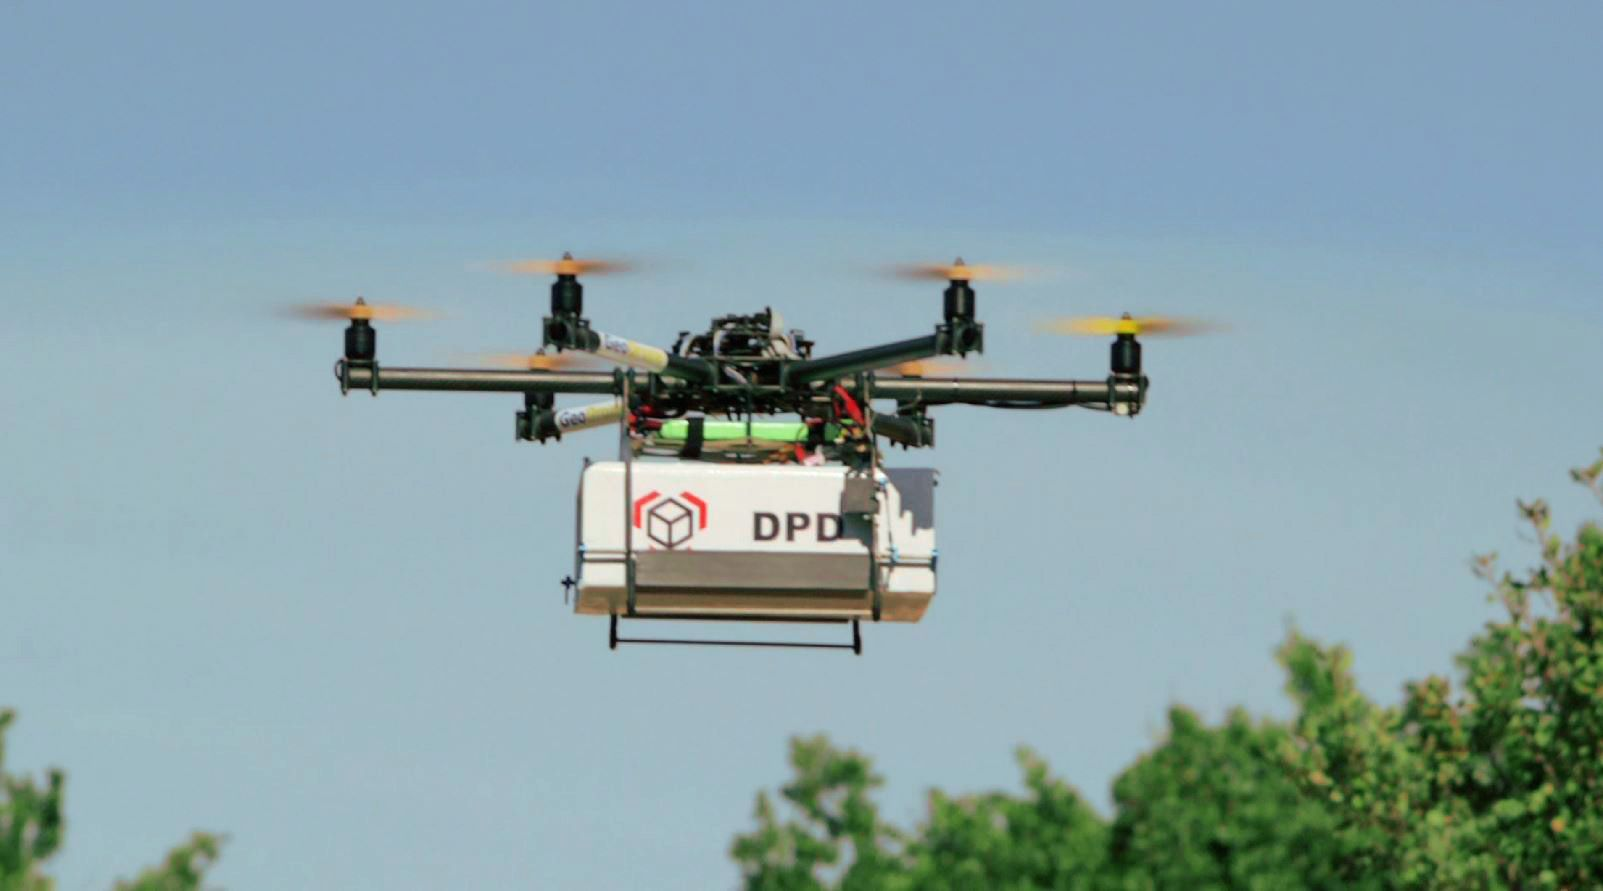
\includegraphics[width=5cm]{images/carrier-drone.jpg} }}%
    \qquad
    \subfloat[A fleet of drones such as on the left, coordinating to move a package from $S$ to $T$ in the least time possible.]{{\includegraphics[width=5cm]{example-image-b} }}%
    \caption{An instance of the Package Handoff problem for a single package}%
    \label{single-pho-example}%
\end{figure}


The challenge is to figure how to get the drones to cooperate to send 
the package from $S$ to $T$ in the least possible time i.e. minimize the makespan
of the delivery process. 

To solve the problem we need to be able to do several things

\begin{itemize}
\item Figure out which subset $S = \{i_1, i_2, \ldots i_k\}$ of the drones are used in the optimal schedule. 
\item Find the order in which the handoffs happend between the drones used in a schedule. 
\item Find the ``handoff'' points when drone $i_m$ hands over the package to drone $i_{m+1}$ for all $m \leq k-1$ 
      \footnote{The final drone $i_k$ in the schedule flies with the package to the target site $T$}
\end{itemize}

This category of problems is a generalization of computing shortest paths in $\mathbb{R}^2$ 
between 
two points. As far as we know such problems have not been considered before in the 
operations research or computational geometry literature; it is, however, reminescent of 
the Weighted Region Problem \cite{mitchell1991weighted} (henceforth abbreviated as 
\texttt{WRP}) where one needs to figure out how to compute a 
shortest \textit{weighted} path between two points in the plane
that has been partitioned into convex polygonal regions, each associated with a constant 
multiplicative weight for scaling the euclidean distance between two points 
\textit{within} that region.  


The distinctive feature of this problem and its generalizations is figuring out how 
to make multiple agents of \textit{varying} capabilities  located at different points 
in $\mathbb{R}^2$ (such as maximum capable speed, battery capacity, tethering constraints 
etc.) \textit{cooperate} in transporting one or more packages most efficiently 
from their given sources to their target destinations. 

While we are framing these problems in terms of drones, one can also apply this problem 
in routing a fleet of taxis to get passengers from their pickup to their dropoff locations. 
Interesting problems might arise in this scenario itself (e.g. what if the sequence of 
pickup and dropoff locations for passengers happen in an online manner, say when passengers request or cancel rides with their 
smartphones?) We leave the investigation of these latter fascinating problems for future work. 
All problems considered in this article are in the offline setting. 


Each chapter in this document is devoted to developing algorithms for a specific 
variant of the package handoff problem (henceforth abbreviated as \texttt{PHO}), beginning 
with the plain-vanilla single package handoff problem described above. 
For most algorithms we will also be giving implementations in Python described in a 
literate-programming style \footnote{Which essentially means you will see code-snippets interleaved with the actual explanation of the algorithms. 
The code snippets are then extracted using a literate programming tool (using a so-called a ``weaver'' and ``tangler'') into an 
executable Python program} \cite{knuth1984literate} using the NuWeb literate programming tool \cite{briggs2001nuweb}  
for weaving and tangling the code-snippets. 

You can check out the Package Handoff code from the following GitHub repository: 

\begin{center}
\url{https://github.com/gtelang/PackageHandoff_Python}
\end{center}

The \texttt{README} file in the repository gives instructions on how to run the code and any of the associated experiments. 
%-----------------------------------------------------
\chapter{Single Package Handoff}
\label{chap:single-package-handoff}

In this chapter, we consider the problem posed at the beginning of the Overview chapter. For convenience
we state the problem again below

\begin{displayquote}
Given the positions $P_i$ of $n$ drones (labelled 1 through $n$) 
in $\RR^2$ each capable of a maximum speed of $u_i \geq 0$. Also given is a package present 
at $S$ that needs to get to $T$. Each drone is capable of picking up the package and 
flying with speed $u_i$ to another point to hand the package off to another drone (which in turn 
hands the package off to another drone and so on). 
 
Find the best way to coordinate the movement of the drones to get the package from $S$ to $T$ in the least 
possible time i.e. minimize the makespan of the delivery process. 

\end{displayquote} 


Note that in the optimal schedule, it is easy to construct an example such that not all drones will necessarily participate
in getting the package from $S$ to $T$. The challenge is to figure out which subset of drones to use, 
along with the handoff points. 

However, the following observations are crucial for the development of algorithms in this chapter. 

\begin{flem}

\begin{itemize}

   \item  For the single delivery package handoff problem,  a slower drone, 
          always hands off the package to a faster drone, in any optimal schedule. 
   
    \item All drones involved in the optimal schedule start moving at time $t=0$. The drone not involved 
          can remain stationary since they don't participate in the package transport. 
     
    \item No drone waits on any other drone at the rendezvous points in any optimal schedule. i.e. if two drones rendezvous at some 
          point $H$, they arrive at $H$ are precisely the same time on the clock. 

    \item The path of the package is a monotonic polygonal curve with respect to the direction $\overrightharp{ST}$
          no matter what the intial positions $P_i$ or speeds $u_i$ of the drones. 
\end{itemize}  


 \end{flem}

Thus, once we \textit{know} which drones participate in the schedule, the order in which they participate in the handoff
from start to finish is determined according to their speeds, sorted from lowest to highest. \footnote{This property is unfortunately 
not true when there are multiple packages to be delivered to their respective desitinations, even for the case where the sources
and targets for all the packages are the same. Examples where this happens are given in the next chapter.}

Before proceeding, we first fix some notation: 

\begin{itemize}
\item $(P_i, u_i)$ for $1 \leq i \leq n$ where $P_i \in \RR^2$ and $u_i \geq 0$, $S,T \in \RR^2$ respectively stand for the initial positions, speed, and source and target points for a package. 
\item $(S=H_{i_0}), H_{i_1} \ldots H_{i_k}$ for $0 \leq i_0, \ldots i_k \leq n$ stand for points where the drones with labels $i_0, \ldots i_k$ handle the package in that oder. More precisely 
      $H_{i_j}$ is the point where drone $i_{j-1}$ hands off the package to drone $i_j$ for $1 \leq j \leq k$.  
\end{itemize}





\section{Propagating Wavefront Algorithms}




The algorithms in this section are inspired by the Continuous Dijkstra paradigm used in computing shortest paths for the Weighted Region Problem
and for computing euclidean shortest paths in the presence of polygonal obstacles \cite{mitchell1991weighted, mitchell1996shortest}. 
The approximation and locality properties of these heuristics are considered later in the chapter. 




The general idea is simple: consider expanding circular wavelets centered at the positions $P_i$, each expanding with speed $u_i$. The drones invovled in the schedule
are then calculated by observing how the wavelets interact in time. The various heuristics differ according to how the subset of drones involved in the delivery 
process is figured out based on nature of the ``wavefront'' used to keep track of the current tentative location of the package. 

Once this subset of drones is calculated,  we use convex optimization (via the convex optimization modelling language CVXPY \cite{diamond2016cvxpy}) 
to figure out \textit{exactly} the handoff points for the drones involved in transporting the package from the source to the destination. 

Precise details follow in the subsections below.


\begin{algorithm}[H]
\SetAlgoLined
\KwData{$(P_i, u_i)$ for $1 \leq i \leq n$ where $P_i \in \RR^2$ and $u_i \geq 0$, $S,T \in \RR^2$  }
\KwResult{ A polygonal path $(S=H_{i_0}), H_{i_1} \ldots H_{i_k}, T$  representing the path travelled by the package. }
      
initialization\;
\While{not at end of this document}{
read current\;
\eIf{understand}{
go to next section\;
current section becomes this one\;
}{
go back to the beginning of current section\;
}
}
\caption{How to write algorithms}
\end{algorithm}




\newpage
\section{Chapter Index of Fragments}
None.

\section{Chapter Index of Identifiers}
 
%------------------------------------------------------






\bibliography{packagehandoff-main} 
\bibliographystyle{ieeetr}


\begin{appendices}
\end{appendices}

\end{document}
